% Created 2013-12-20 金 04:52
\documentclass[12pt]{jsarticle}
\usepackage[dvipdfmx]{graphicx}
\usepackage{comment}
%\usepackage{setspace}
%%\date{\today}
%\title{}
\textheight = 25truecm
\textwidth = 18truecm
\topmargin = -1.5truecm
\oddsidemargin = -1truecm
\evensidemargin = -1truecm
\marginparwidth = -1truecm
\def\theenumii{\Alph{enumii}}
\def\theenumiii{\alph{enumiii}}
\def\labelenumi{(\theenumi)}
\def\labelenumiii{(\theenumiii)}
%\setstretch{0.9}
\begin{document}

%\maketitle
%\tableofcontents

\begin{center}
%%%%%%%%%%%%%%%%%%%%%%%%%%%%%%%%%%%%%%%
%%%タイトル                         %%%
%%%%%%%%%%%%%%%%%%%%%%%%%%%%%%%%%%%%%%%
{\LARGE 2014年度後期研究計画(藤田)}
\end{center}

\begin{flushright}
  2014/9/04\\
  藤田将輝
\end{flushright}
%%%%%%%%%%%%%%%%%%1章%%%%%%%%%%%%%%%%%%%
\section{はじめに}

本資料では藤田将輝の研究テーマの概要と2014年度後期研究計画案,およびその後の課題案について述べる.


\section{自身の研究テーマ(案)}
\begin{itemize}
\item[(題目案)] {\bf Mintを用いた割り込み処理のデバッグ手法の提案(案)}

\item[(概要案)] OSのバグの中には割り込みタイミングに依存するバグや,割り込みレベルの違いによって発生するバグが存在する.
バグの特定にはバグの状況を再現する必要があるが,割り込みは非同期的な処理であるため,
そのバグを再現するのは困難である.
このデバッグを支援する手法としてVMを使ったものがある.
VM上で2つのOSを走行させ,一方のOSから他方のOSへ意図的に割り込みを発生させることでバグの状況を再現し,デバッグを支援するものである.
しかし,VMを使った方法ではVMとハイパーバイザの間の処理の遷移に伴う処理負荷が発生するため,一定間隔で発生する割り込みや,
短い間隔で発生する割り込みに対するバグのように,処理負荷が影響する割り込み処理のデバッグが困難である.
そこで,Mintを用いたデバッグ手法を提案する.
Mintは仮想化を用いずに,1台の計算機上で複数のOSがCPU,メモリ,およびデバイスを分割占有して走行するため,ハイパーバイザによる
処理負荷が存在しない.
このため,どのようなタイミングの割り込みであっても再現することが可能である.
任意のタイミングで任意の割り込みレベルの割り込みを発生させ,バグの状況を再現し,デバッグを支援する機構を実装する.
\end{itemize}
\section{特別研究報告書に向けた研究テーマ(案)}
特別研究報告書に向けて,任意のタイミングで連続で割り込みを発生させ,デバッグを支援する手法を実装する.
具体的にはMintを用いてNICドライバに任意のタイミングで割り込みを発生させる機構を実装する.
割り込み元のOSからNICドライバの割り込み処理に必要なデータを共有メモリに格納し,割り込み元のOSが占有するコアから割り込み先のOSが占有している
コアへIPIを送信することで割り込みを発生させる.
また,2章との差は割り込みレベルの違いによって発生するバグを考慮するか否かであり,特別研究報告書に向けての研究では
割り込みレベルの違いによって発生するバグは考慮しない.
題目案と概要案を以下に示す.
\begin{itemize}
\item[(題目案)] {\bf Mintを用いたNICドライバへの割り込み挿入手法の実現(案)}
\item[(概要案)] OSのデバッグ手法としてVMを用いたものがある.これはVM上で2つのOSを走行させ,
一方のOSから他方のOSへ任意のタイミングで割り込みを発生させ,バグを再現し,デバッグを支援するものである.
しかし,VMを使ったデバッグ手法では,VMとハイパーバイザ間の処理の遷移に伴う処理負荷が発生する.
このため,一定間隔で発生する割り込みや短い間隔で発生するバグのように処理負荷が影響する割り込み処理のデバッグが困難である.
そこで,Mintを用いたOSのデバッグ手法が提案されている.
Mintは1台の計算機上で複数のOSが計算機資源を分割占有して走行できる.
本研究では,Mintにおいて,NICによる割り込みを任意に挿入できる環境を実現する.
具体的には,割り込み元OSからNICの割り込み処理に必要なデータを共有メモリに格納し,割り込み元OSが占有しているコアから
割り込み先のOSが占有しているOSへIPIを送信し,割り込み処理を発生させるものである.
これにより,NICドライバの,割り込みにより発生するバグを再現し,デバッグを支援することができる.

\end{itemize}



\section{今後の予定(案)}
今年度の予定を図1と別紙の2014年度課題一覧表(藤田)に示し,以下で説明する.
なお,それぞれの項目の最後に別紙の2014年度課題表一覧と対応させた通番を記す.

\begin{enumerate}
\item IPI送受信時の処理の調査
\begin{enumerate}
\item IPI送信に関連するレジスタの調査(通番1) 
\item IPIを送信するシステムコールの作成(通番2)
\item 割り込みハンドラを登録するシステムコールの作成(通番3)
\item sleep関数を用いずに連続でIPIを送信した際に割り込みハンドラが実行されない原因についての調査(通番4)
\item IPI送信間隔を調整するために使用しているndelay関数による遅延時間の正確さの調査(通番5)
\item IPI送信に失敗した際の処理の調査(通番6)
\end{enumerate}

\item Linuxテストの調査
\begin{enumerate}
\item Linuxテストの収集と分類(通番7)
\item デバッグ手法の調査(通番8)
\end{enumerate}

\item VND(Virtual Network Device)方式によるOSnode間通信機能の実現
\begin{enumerate}
\item NICデバイスドライバの解析(通番9)
%\item VND方式によるOSnode間通信機能の検討
\item NICデバイスドライバが発行したI/O命令をフックする方法の検討(通番10)
\item 使用する共有メモリ領域の検討(通番11)
\item 受信バッファへのパケットの格納(通番12)
\item パケット受信割り込みの生成(通番13)
\item VND方式によるOSnode間通信機能の設計と実装(通番14)
\end{enumerate}

\item 評価
\begin{enumerate}
\item ソースコードの改変量の調査(通番15)
\item 大量パケットの連続送信によるストレステスト(通番16)
\item 仮想計算機を用いた割り込み処理のデバッグ支援環境の作成(通番17)
\item 割り込み時のオーバヘッド,割り込みタイミングの精度(通番18)
\end{enumerate}

\end{enumerate}

\begin{figure}[t]
\begin{center}
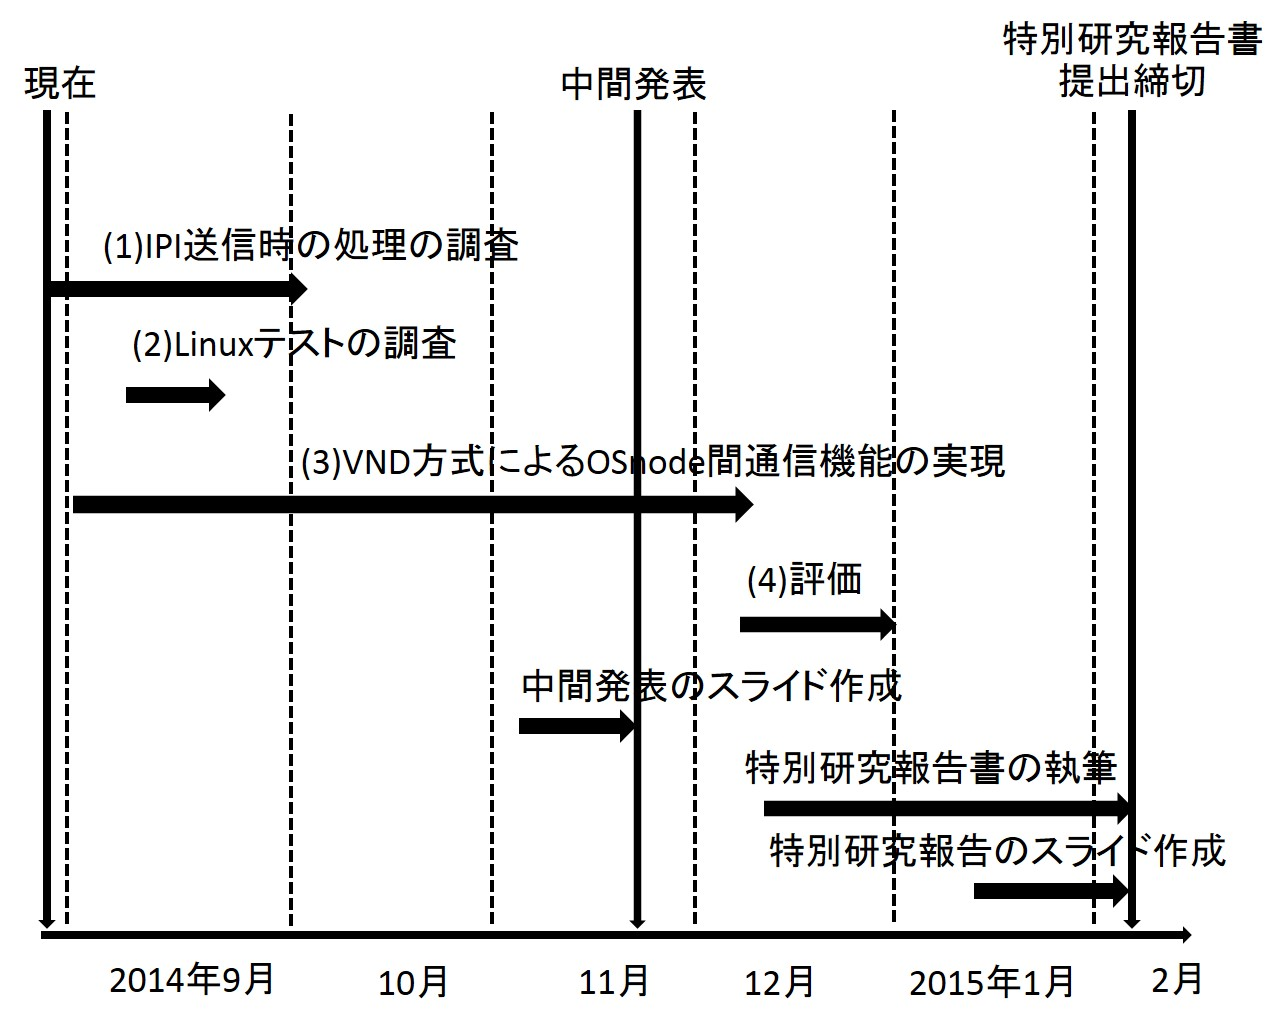
\includegraphics[height=8.0cm]{./fig1.jpg}          
\caption{2014年度後期研究計画}
\label{fig:up}
\end{center}
\end{figure}


\section{特別研究報告後の予定}
特別研究報告後の研究内容を以下に記述する.
OSのバグには割り込みレベルの違いによって発生するバグが存在する.
このバグを再現し,デバッグを支援する機構を作成する.
特別研究報告後の予定を以下に示す.
なお,それぞれの項目の最後に別紙の2014年度課題表一覧と対応させた通番を記している.
\begin{enumerate}
\item デバッグ手法の実装
\begin{enumerate}
\item 各割り込みの割り込みレベルの調査(通番19)
\item 割り込みレベルの違いによって発生するバグの調査(通番20)
\item 割り込みレベルの違う複数の割り込みを同時に発生させ,バグを再現する機構の実装(通番21)
\end{enumerate}
\end{enumerate}



\section{おわりに}
本資料では,藤田の2014年度後期研究計画について記述した.


\end{document}
